\section{ECS Literature Review}
\label{chap:1}

Historically, the documented first ECS was introduced in 1998 with the game titled "Thief: The Dark Project".\cite{RomeoPHD} The studio's motivation behind attempting an alternative to OOP was that they found OOP introduced massive class hiearchies, deep inheritance paths, and highly specialized code. In an attempt to streamline their project, they developed the first ECS.\cite{Haerkoenen2019} Apple, in their documentation for their personal ECS, specifically states "Inheritance-Based Architecture Hinders Game Design Evolution" and provides examples and reasoning why similar to the points given above.\cite{AppleECSBad}

The ECS pattern argues from the position that it can solve development issues by limiting the hierachy to contain only three layers. And thus it is classified as an architectural pattern under Data-Oriented Design (DOD).\cite{RomeoPHD} To this day, ECS maintains its importance in simulations. For example 16 years after Thief came out, Apple in 2015 introduced an implementation of ECS into their GameplayKit API framework. \cite{AppleECS}

Scientific literature on the topic of ECS's were limited and hard to find. Although there is not much scientific literature, there are still many articles, conferences, and well-documented libraries from respected individuals in the games industry used as references. GECS is inspired by the articles written by Sander Mertens, the creator of the very popular FLECS framework and can be found in \cite{SanderMertensECS}. 

For future reference, there is a table in Appendix \ref{appendix:a} dedicated to providing definitions of ECS concepts and concepts introduced in this paper.

\subsection{Motivation \& The Weaknessess Of Object Oriented Programming}

It has been exhaustively shown that Object-Oriented Programming increases the difficulty of achieving desired simulation goals and that there are plenty attractive alternatives. The two main weaknesses that an ECS intends to solve is: poor cache utilization and poor parallelization.\cite{RomeoPHD}

Large game development projects deep into using OOP principles learn quick how hard it is to keep important data cached and keep junk out. OOP hiearchies are generally connected with pointers, allowing for an easy pathway to pointer abuse by library users and developers in general. ECS proposes a solution to this by introducing the concept of components. All definitions within this paper are documented in Appendix \ref{appendix:a}. Since components are detached from their owner, the entity, we as engine designers can place these compnents in memory however we please. It's not an uncommon practice to see component data be stored in long, contiguous, homogeneous vectors. Suppose there exists a type \texttt{Vec2} that contains the coordinates of all entities within the ECS. If all entities have their \texttt{Vec2} positions layed contiguous in memory, then the data is primed to be very cache friendly. \cite{Wiebusch2012}\cite{SanderMertensECS} This scenario also has a concurrency advantage since using SIMD instructions, for example, is possible. 

It's also important to note that parallelism while using OOP can be very painful due to synchronization requirements over memory that was not engineered to effectively be parallelized. Because ECS's follows principles from Data-Oriented Design, ECS's can generally produce code that is more parallelizable by default.\cite{RomeoPHD}

\subsubsection{Introduction To ECS}
For something to classify as an Entity Component System, it must contain the three properties present in its name. This paper will present two alternative ECS architectures to gain some familiarity. 

It does not matter how or where each concept is used or placed in the design. Entities are identifiers, components are data, and systems connect the two. This gives a large amount of room for designing interesting and unique architectures that can solve specific performance needs without much interference to the end users. 

One popular and easy to build approach is shown below in figure \ref{fig:naive1}, where entities encapsulate their own data. This diagram shows an ECS architecture that is close in concept to OOP. Each entity contains certain data elements, and based on these elements, the entities are filtered into systems that operate on them. It's important to note that the diagram states "Some parallelized behavior" below each filter but does not specify how. The Render System and Spawning System both use the \texttt{Position} component. \texttt{Render} is most likely only reading the available positions and \texttt{Spawning} only creates new \texttt{Position} components. As a designer, one must be careful specifying what sort of concurrent guarantees exist within the architecture. 

\begin{figure}[H]
    \centering
    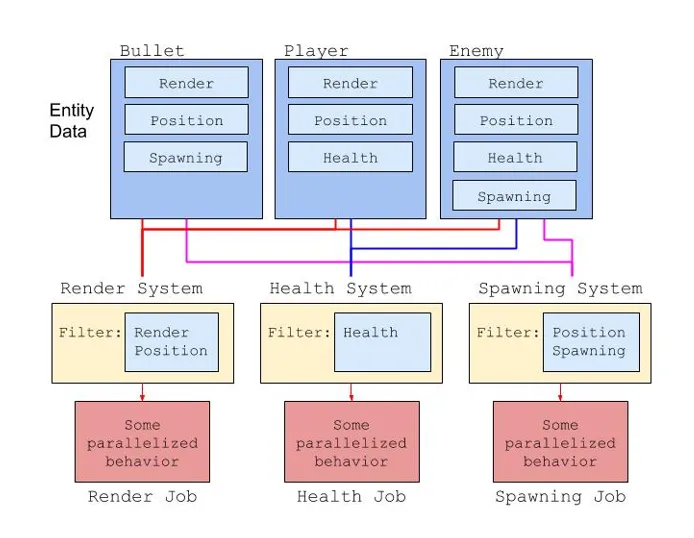
\includegraphics[width=0.7\linewidth]{resources/naive_ecs2.png}
    \caption{Simple ECS Architecture (OOP Inspired)}
    \label{fig:naive1}
\end{figure}


The following in figure \ref{fig:advanced2} is a more advanced ECS architecture designed specifically for concurrency in mind via the integration of wait-free hash maps.\cite{waitfreemapsecs} In this more intelligent architecture, notice how entities are decoupled from their components. Entities are organized into their own category type. Systems then concurrently request from sets of hash maps containing component data separately.

\begin{figure}[htbp]
    \centering
    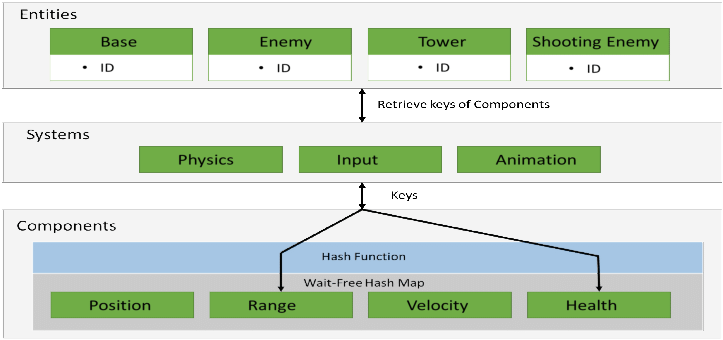
\includegraphics[width=0.7\linewidth]{resources/ecs2.png}
    \caption{ECS Architecture}
    \label{fig:advanced2}
\end{figure}

Both architectures in \ref{fig:naive1} and \ref{fig:advanced2} are valid ECS architectures that have their own performance tradeoffs and gains. I would imagine in the first architecture, that unique entity lookups may be faster because entity data is grouped together while batch component processing may be faster in the second. 

\subsection{Naive Entity-Component System Model}
\label{sec:ecs_naive}
The following section discusses a thread-unsafe naive implementation of an ECS to give a deeper understanding on how such an architecture works. The naive implementation is presented in the C language the same as the GECS Library. The full naive code is given for study in appendix \ref{appendix:b}.

\subsubsection{Naive Data Structures}
The implementation style used for this ECS is referred to as a Dense ECS. \cite{EnTT_SparseSets} A Dense ECS is a style that orders components and entities in memory into a table-like structure such that entities and components are the table rows and columns. It's up the the engine designer to decide if the entities or components should be optimized for look-up when using a Dense ECS. In the naive version provided, the components are vectorized.

There are four core properties within the ECS structure:

\begin{figure}[H]
\begin{lstlisting}[
    language=Java,
    numbers=none
]
struct ecs {
  int32_t           id_gen;     /* Generates unique IDs */
  entity_map        entities;   /* Contains all entity info */
  component_map     components; /* Contains all component data */
  ecs_systems       systems;    /* Vector of all the systems */
  stalloc          *alloc;      /* The allocator for this ECS */
};
\end{lstlisting}
    \caption{Naive ECS Members}
    \label{code:naive_ecs_data}
\end{figure}

Starting from the top, \texttt{id\_gen} is used to generate unique IDs for this ECS instance. Unlike the GECS library that uses hashes to collect components, this implementation shares incrementally generated IDs from \texttt{id\_gen} between entities and components.

The \texttt{entities} member is a mapping between an entity ID and an intermediary type the \texttt{component\_indexer}. This indexer is another map that takes a given component ID and returns the position within a vector of this specific entities component. This transformation can be formally expressed as:
\begin{equation*}
    f(a, b) : Map(a) \rightarrow Map(b) \rightarrow Int
\end{equation*}

This isn't the worst performance in the world, but notice that locality is affected heavily since there are two map jumps required to get the position of an entities component. Engines that intend to do lots of entity lookups are not advised to be engineered this way. 

The \texttt{components} member is a mapping between a component ID to a homogeneous vector of those components. This can be fed directly to the library user to do fast operations or a specific position in this component can be loaded by the entity routine described above.

The \texttt{systems} member is a vector containing information required to run a system. The requirements to run a system in an ECS, as described in the appendix \ref{appendix:a}, is some function and a list of required types. 

Note how there are already many opportunities to parallelize operations over the component vectors returned from the \texttt{components} map.

\subsubsection{Naive Entity Operations}
In order to create a new entity, the following steps are taken:
\begin{enumerate}
    \item Increment \texttt{id\_gen}
    \item Allocate \texttt{i} $\leftarrow$ \texttt{component\_indexer} 
    \item Store in map \texttt{entities} $\leftarrow$ \texttt{i}
    \item Return \texttt{id\_gen}
\end{enumerate}

In order to perform add, create, modify, or delete operations of components owned by a single entitiy, the \texttt{component\_indexer} of the entity must be loaded to retrieve the entities position in the component vector.

\begin{enumerate}
    \item Load \texttt{e} $\leftarrow$ \texttt{entities}
    \item Load \texttt{c} $\leftarrow$ \texttt{components}
    \item Load \texttt{p} $\leftarrow$ \texttt{e.get(comp\_id)}
    \item Load \texttt{y} $\leftarrow$ \texttt{c.at(p)}
    \item Perform single component operation on $y$
\end{enumerate}

As can be seen in the two algorithms above, a Dense ECS is not designed for modifying a single entity at a time but many all at once. So, single entity accesses are intentionally slower that component accesses. \cite{EnTT_SparseSets}

\subsubsection{Naive System Operations}
A core feature of an ECS implementation is for the ability to query systems based on what components entities. Based on this information, each registered system will collect pointers to which vectors it will process.

When registering a system:
\begin{enumerate}
    \item For each component ID \texttt{comp id} $\leftarrow$ \texttt{components} such that \texttt{comp id} $\in$ 
    
    \texttt{system\_data.requirements}
    \item Save \texttt{comp id} $\rightarrow$ \texttt{system\_data.to\_process }
\end{enumerate}

Now all that needs to be done is once per tick, each system runs once with their components ready to be processed.

\subsubsection{Naive Demo}
The naive ECS code in appendix \ref{appendix:b} comes attached with an example demo project. The project is a simple simulation that sets two entities positions to be above the ground in a 2D space and for each tick, the entity falls by one unit. When the entity reaches the ground, their component is deleted. When both entities have reached the ground, the simulation ends. 

The motivation behind deleting the component is that the naive ECS returns \texttt{NULL} when asking for a component from an entity that does not exist. So it's easy to check if the entity has reached the floor or not by checking for the existence of the \texttt{Vec2} component. This component deletion also prevents the entities from having their y-coordinate from going negative.

\subsection{Existing ECS And Implementation Styles}
From part \ref{chap:1}, its easy to surmise that the ECS pattern can be implemented in many different ways, giving way to unique performance benefits and tradeoffs per style. This section covers an overview of various implementation styles discovered around ECS architectures. This list is not exhaustive and includes only ones that were found in the research phase of this paper. 

\subsubsection{Entity ID Styles}
A lot can be done with just reserving a couple bits on IDs generated. The popular ECS framework called FLECS, short for Fast Lightweight Entity Component System, proposes to represent all component ID's generated in the same manner entity ID's are generated. 

In the GECS C Libary implementation, entity ID's and component ID's use different generation techniques. Entity ID's are generated the traditional way using an incrementing counter but component ID's are actually hashes produced by the typename. The hashing function used by GECS is djb2 \cite{hashing}, a nice and fast hashing function that has decently low collision probability. It has been slightly adjusted from the authors version found online to consume an arbitrary amount of bytes based on the \texttt{void *} type but nonetheless is the same algorithm. 

FLECS splits a \texttt{uint64\_t} into two parts where the lower 32 bits represents the entity and the upper 32 bits are reserved for optimizing internal ECS mechanisms. The following are three styles that can take advantage of this smart ID system to improve runtime performance.

\begin{figure}[H]
    \centering
    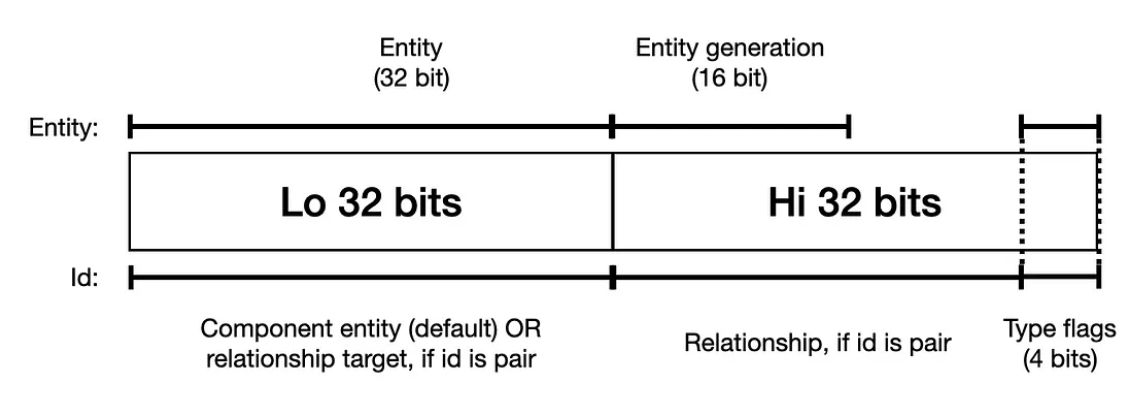
\includegraphics[width=0.5\linewidth]{resources/entity_generation.png}
    \caption{Smart Entity Generation in FLECS}
    \label{fig:entity_generation}
\end{figure}

\textbf{Runtime Tagging:}
A tag in an ECS is a component with no data. Tags are used generally to apply entities to systems without the intent of editing any data based on the tag, but the components adjacent to it. Since components and entity ID's are indistinguishable, entities can share direct relationships to other components via runtime tagging as shown in the example below. \cite{RomeoPHD}

\begin{figure}[H]
    \begin{lstlisting}[
        language=Java
    ]
component CloseCircle = world.component();
entity John = world.entity();
entity Mary = world.entity();
entity Brad = world.entity();
CloseCircle.add(John, Mary, Brad);
CloseCircle.each([](entity friend) { /* John, Mary, and Brad */ });
\end{lstlisting}
    \caption{Runtime Tagging Example}
    \label{code:runtime_tagging}
\end{figure}

The code in figure \ref{code:runtime_tagging} on line 5 is when the ID of \texttt{CloseCircle} is modified to contain some direct relationship to the entities $[\texttt{John}, \texttt{Mary}, \texttt{Brad}]$. Usually such a relationship is impossible since only entities contain components, but in this case the situation is reversed: components contain entities. This is possible because entities and components have the same ID properties for runtime tagging.

\textbf{Reflection:}
The upper 32 bits can be used for reflection. Reflection is the ability to serialize component data out of the ECS. Serialization can be done by constructing a new component to house other components as if it were an entity.

This is similar to the code found in Figure \ref{code:runtime_tagging} but if all the entities (John, Mary, Brad) were components instead of entities. Then, all thats needed to be done is log the component data of the serialization component. By doing this, reflection can be achieved with minimal effort. All that is required is to iterate over the components reflected.

\textbf{Entity Liveness:}
A core issue with the ECS pattern is that many games will burn through ID's fast. As such, recycling IDs is important part of an ECS implementation. FLECs reserves the first 16 bits of the upper 32 bits of entity identifiers as a generation count. So a counter for the counter of how many times this ID has been recycled. This allows for easy checking if an entity is still alive.  

\textbf{Entity Relationships:}
One of the biggest flaws of ECS architectures is that perfoming direct entity relationship queries are slow and not performant because of how components and entities are organized. By adding relationships to other entities in the ID, query times can shorten. For more information on how this is done inside FLECS, which pioneered this techinque, read Sander Merterns article in \cite{SanderMertensEntityIDs}.

\subsubsection{Dense ECS}
\begin{figure}[htbp]
    \centering
    \begin{verbatim}
        Entities         +-----+-----+-----+-----+-----+  
        Are Rows         |  A  |  B  |  C  |  D  |  E  |  
                   +-----+-----+-----+-----+-----+-----+  
        Components |  0  |  -  |  -  |  +  |  -  |  -  |  
        Are Cols   +-----+-----+-----+-----+-----+-----+  
                   |  1  |  +  |  -  |  +  |  -  |  +  |  
                   +-----+-----+-----+-----+-----+-----+  
                   |  2  |  -  |  +  |  +  |  -  |  -  |  
                   +-----+-----+-----+-----+-----+-----+  
                   |  3  |  +  |  -  |  -  |  +  |  -  |  
                   +-----+-----+-----+-----+-----+-----+  
                   |  4  |  -  |  -  |  -  |  +  |  -  |  
                   +-----+-----+-----+-----+-----+-----+                                 
    \end{verbatim}
    \caption{Dense ECS Architecture Table Example}
\end{figure}

Dense ECS's, also known as Table based ECS's, store entities inside of large tables. In these tables, components and entities are columns and rows respectively. This gives way to fast component or entity queries, depending on which is is contiguous in memory. Some popular types of this ECS is FLECs or the Unity Game Engine's own ECS, Unity DOTS. \cite{SanderMertensFAQ}

\subsubsection{Sparse ECS}
To understand Sparse ECS architectures, a small introduction into an exotic data structure is necessary. A Sparse Set is a datastructure dedicated to keeping the invariance of the following property:
\begin{equation*}
    \forall v \in \{0,\ldots, n-1\} : \text{D}[S[v]] = v
\end{equation*}
In the property above, $D$ and $S$ represent two vectors. The dense vector and sparse vector respectively. By using these two vectors in unison: lookup, insertion, and deletion time are all $O(1)$ and iteration through the set is $O(n)$. Interestingly enough, this data structure is one that does not require memory to be initialized \cite{sparse_profit}. The only downside to Sparse Sets is that they must be capable of representing an entire domain since direct index access is used. If, for example $v = 10000$, then there must be at least $10000$ elements in $S$. $D$, the dense vector, will always be the length of the set itself.

The main advantage of sparse ECS implementations is how fast it is to test if an entity contains a component. Because of this, sparse ECS's advantages come in the form of query optimization. In a sparse ECS, a query collects entities by roughly performing the following algorithm: queries all entities on each sparse set. If the entity is in that sparse set, then add to the query. Bitset ECS's are known to use also similar approaches in their implementations.\cite{EnTT_SparseSets}

Sparse sets also have another use where systems own their own sparse sets and they are kept to date each tick during runtime. These system owned sparse sets are then used to collect entities related to the system. An example of an ECS that does this technique is ecst. \cite{ecst}

Overall, it's important to know that sparse set ECS's are popular in situations where fast add/remove of single component operations are preferred over efficient batch operations. To back this claim, FLECS which is a popular dense ECS published its own benchmarking data against other industry-wide used ECS's. From their data, FLECS has slower add/remove component operations than EnTT, a popular sparse set based ECS.\cite{FLECS_EnTTCompare} Regardless of the advantages and disadvantages of using sparse vs dense ECS's, it can be summed up nicely by the creator of EnTT \cite{EnTT_archetype_and_quote}:

\begin{quote}
    \textbf{It’s a matter of taste}, in fact.
        - Michele Caini
\end{quote}

\subsubsection{Bitset-based}
Another exotic structure used in ECS implementations are bitsets. A bitset is analogous to a hashset. It tracks if certain indices exist are within a set, but the implementations differ vastly however. Bitsets are known for their memory efficiency and are preferred over hashsets if the set is known to store large volumes of objects in the set. \cite{Sutherland2014}

A bitset-based ECS stores components in contiguous arrays where the entity ID is used to index. The bitset is used in this application to check if the entity contains that component. There are many different flavours of approaches using this style, such as using a hierarchical bitset structures. \cite{SanderMertensFAQ} EntityX is one of the architectures reviewed that uses bitsets.

\subsubsection{Reactive}
A reactive ECS is significantly more different than the others in this list. A reactive ECS uses signals emitted from mutating entities to keep individual lists of which entities belong to which system. Entitas is an example of this. \cite{SanderMertensECS}

\subsection{Concurrency in ECS Implementations}
The majority of ECS implementations investigated had concurrency support but were severely undocumented. So only two were investigated: FLECS and EnTT.

\subsubsection{FLECS}
The concurrency model of FLECS is simple. The user initially sets the amount of worker threads manually, and entities matched with a system will be divided equally across threads. Changes to entities are stored in what Sander Mertens calls a "command queue" that are later merged before the end of the tick.\cite{missing_docs} This system is similar to the concurrency model used for GECS most likely because both GECS and FLECS are Dense ECS's that rely on vectorizing type compositions for concurrency gains.

\subsubsection{EnTT}
The EnTT framework does not do anything special to for concurrent performance gains since their design naturally allows for parallelizable code to be threaded by the user themselves. Michele Caini states in his documentation that "Views, groups, and interators in general aren't thread safe by themselves" but then gives suggestions on how to apply concurrency using their architecture. The author also ends on a note saying that they at least support concurrent entity generation by setting the \texttt{ENTT\_USE\_ATOMIC} flag.\cite{EnTT_multithreading} GECS by default using atomics to coordiante ID generation across threads.